%TODO handout %2 seiten, schriftgre? seitenrand?
%	- alles was in den Folien ist
%	- historie verlngert
%	- formeln
%	- eigenschaften verlngert
% 	- type1 vs 2
%	- hochtemp. outlook [folie?!]
%	- BCS zusammenfassen
%	- technische anwendungen?
%	- flietext statt stichpunkte


\documentclass{beamer}
%\documentclass[trans]{beamer}
\usetheme{Frankfurt}
%\usepackage{german}
\usepackage{textcomp}
\usepackage[utf8]{inputenc} 
\usepackage{url,hyperref}


%\usepackage{pgfpages}
%\pgfpagesuselayout{4 on 1}[a4paper,border shrink=5mm]

%\usepackage[T1]{fontenc}
\beamersetuncovermixins{\opaqueness<-10>{25}}{\opaqueness<5->{0}}
%\setbeameroption{show notes on second screen}




\begin{document}

\title{Superconductivity}   
\author{Benjamin Huber \qquad Carolin Wille} 
\date{28.11.2011}
%\logo{\includegraphics[scale=0.14]{logo-SF}}

\begin{frame}
\titlepage
\end{frame}

%überblick was wir so besrehcen? -_-


\section{Introduction} %2 %c
% what is superconductance
% historic! evtl. hist. plots?

\subsection{Overview}
\begin{frame}{What is Superconductivity?}
\begin{columns}
        \column{.55\textwidth}
        \begin{itemize}[<+->]
\item Low Temperature Phenomenon
\item Loss of Electrical Resistivity 
\item Everlasting Currents
\item Strong Magnetic Fields
\end{itemize}
                
        \column{.45\textwidth}
        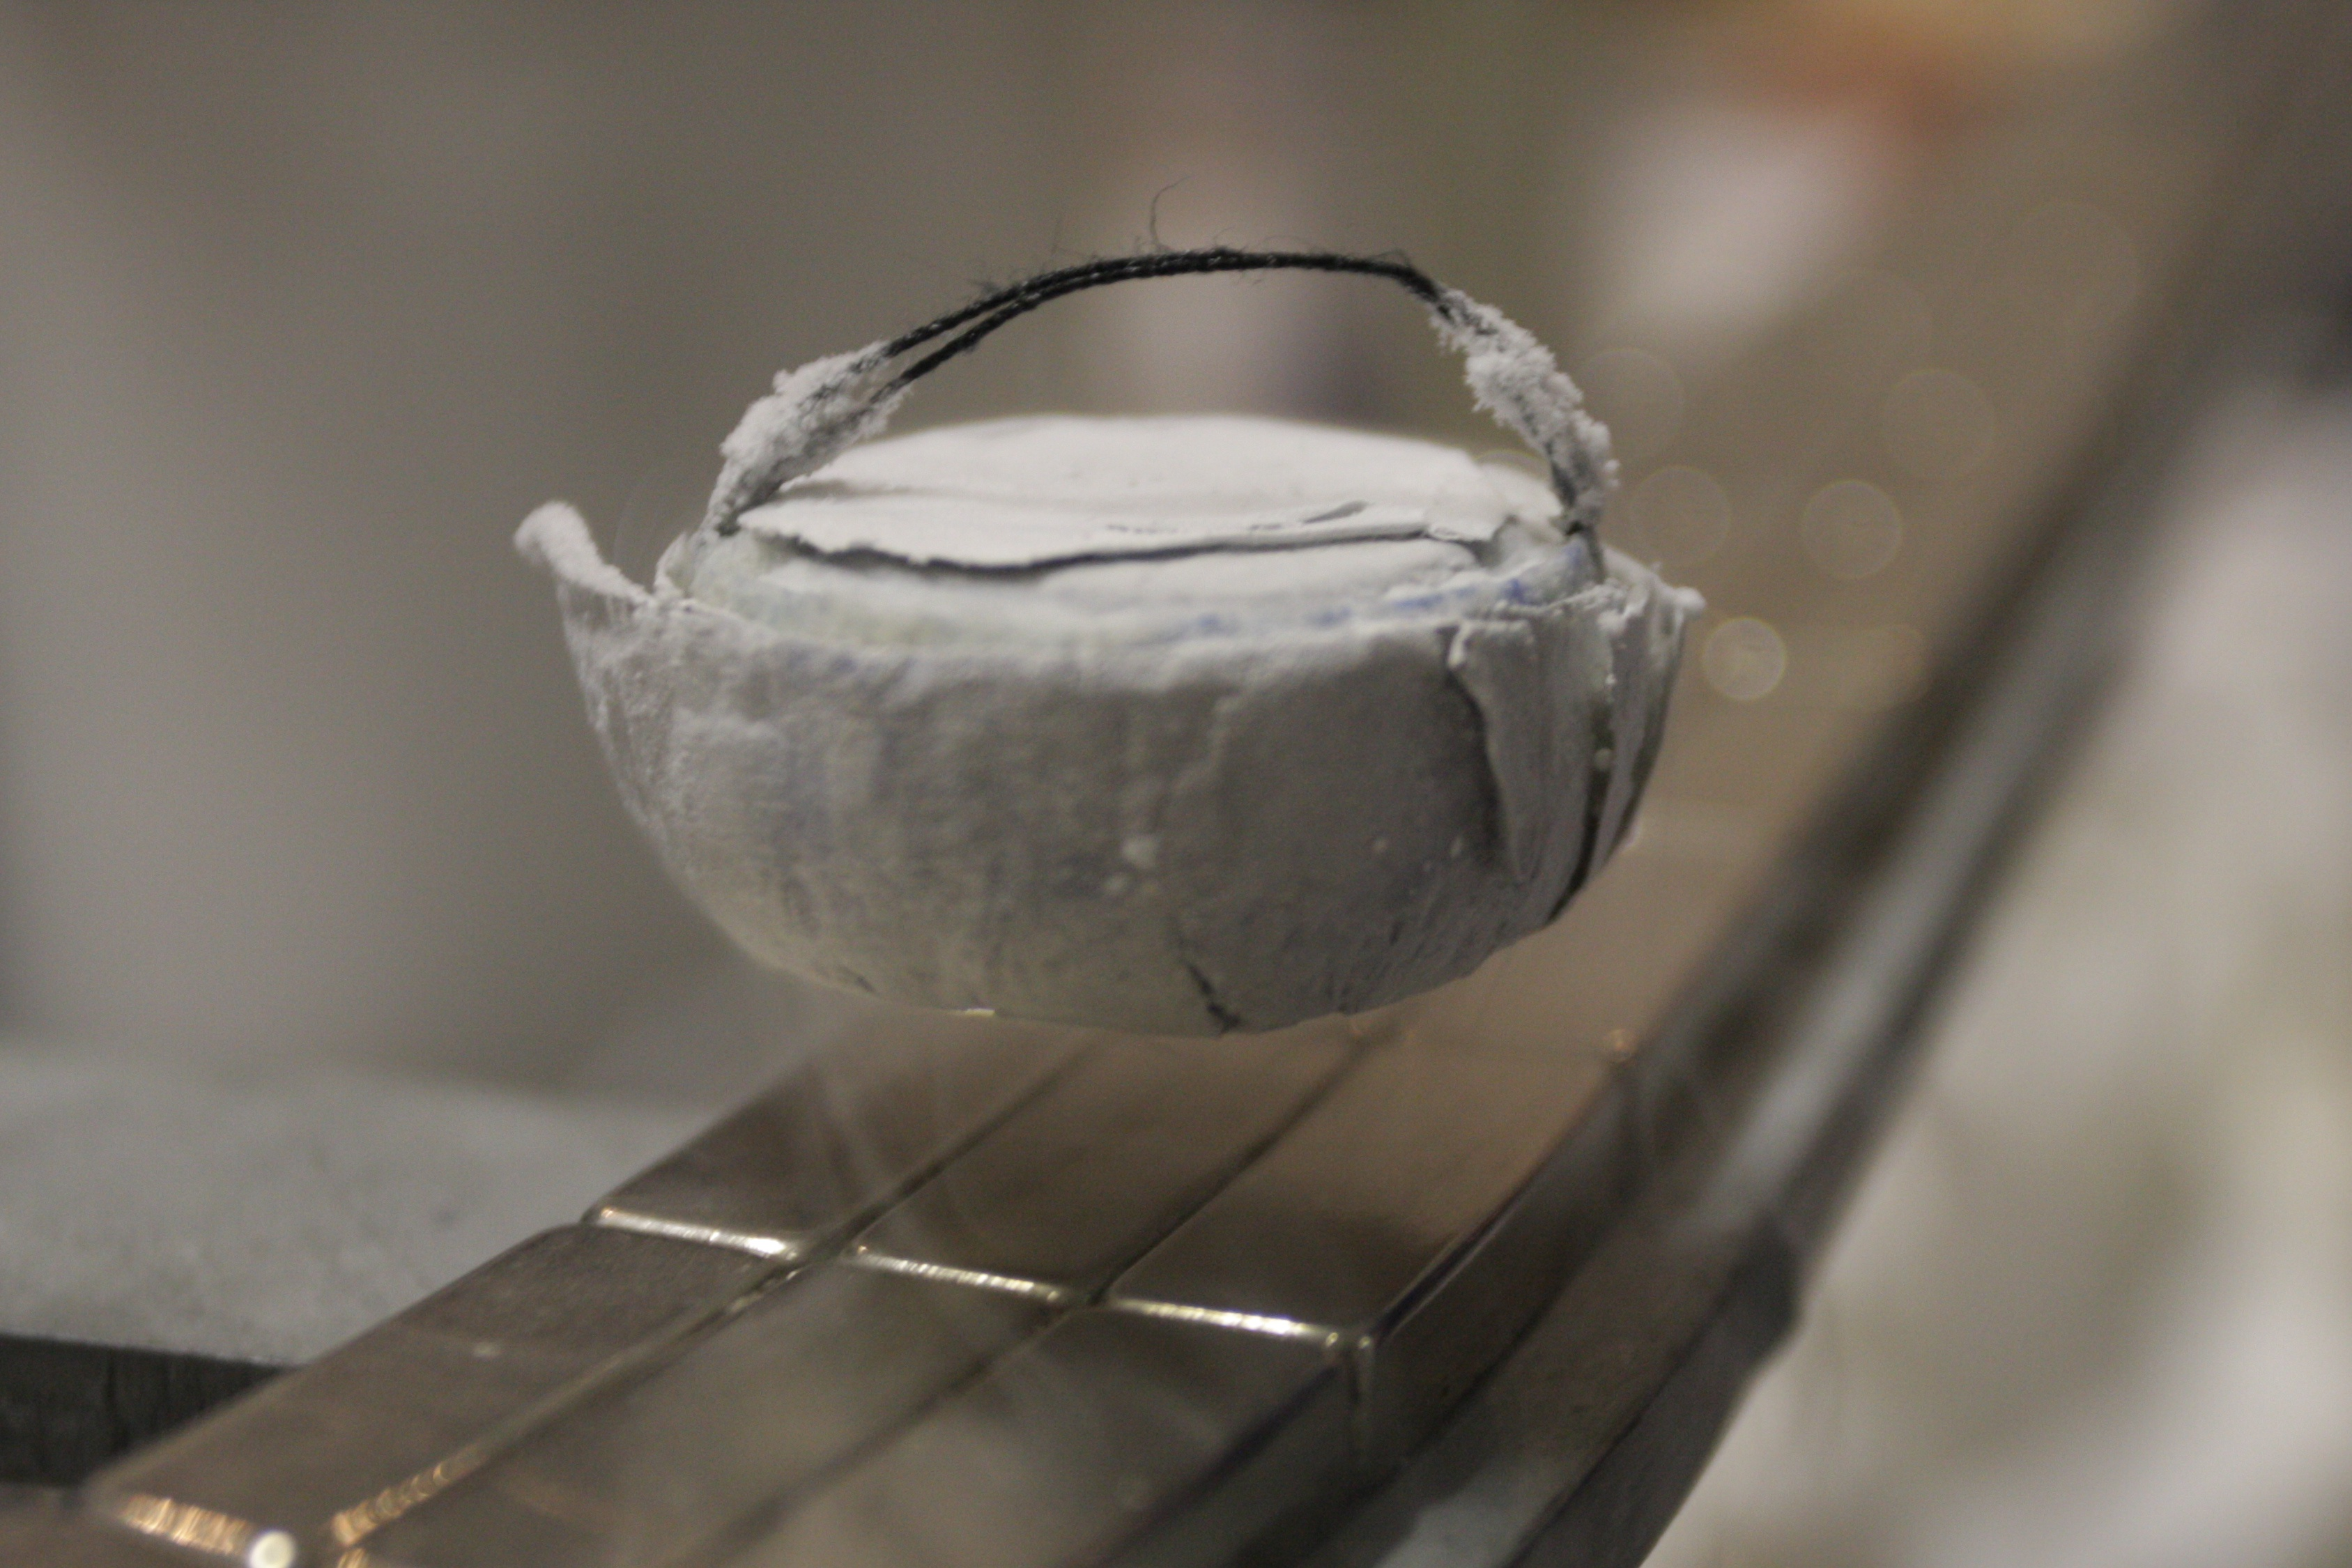
\includegraphics[width=\textwidth]{img/levitation2.jpg}
%\includegraphics<2>[width=\textwidth]{img/heikemess.jpg}
%\includegraphics<3>[width=\textwidth]{binding.jpg}
\end{columns}
        \footnotetext[1]{\tiny Henry Mühlpfordt, TU Dresden, High Temperature Superconductor levitating permanent magnet (2010)}
\end{frame}


\subsection{History}
\begin{frame}{History of Discovery}
\begin{columns}
        \column{.65\textwidth}
        \begin{itemize}[<+->]
\item H. Kammerlingh Onnes, Leiden (1911)
\item Liquid Helium $T<4.2$ K 
\item Measurements of Electric Resistivity
\item "Jump" at critical temperature $T_C$
\end{itemize}                
\column{.4\textwidth}
        \includegraphics<1>[width=0.8\textwidth]{img/heike.jpg}
                
		\includegraphics<2>[width=0.8\textwidth]{img/heike.jpg}
		\includegraphics<3>[width=\textwidth]{img/heikemess.png}
		
		\includegraphics<4>[width=\textwidth]{img/heikemess.png}      
\end{columns}
\footnotetext[1]{\tiny H.K. Onnes: Comm. Leiden 12ßb (1911)}
\footnotetext[2]{\tiny \url{http://nobelprize.org/nobel_prizes/physics/laureates/1913/onnes-bio.htm}}
\end{frame}

\subsection{Properties}
\begin{frame}{Some Properties of Superconductors}
\begin{itemize}[<+->]
\item Critical Temperature
\item Critical Magnetic Field
\item Critical Current
\item ...
\end{itemize}
\end{frame}



\section{Meißner-Ochsenfeld Effect}



\subsection{Critical Field}
\begin{frame}{Critical Magnetic Fields}
\begin{columns}

\column{.45\textwidth}
\begin{itemize}[<+->]
\item \small Critical Temperature $T_C$
\item \small Critical Magnetic Field $B_C$
\item \small $B_C=B_{C0} \left[ 1 - \left(\frac{T}{T_C}\right)^2 \right]$
\end{itemize}    
            
\column{.6\textwidth}
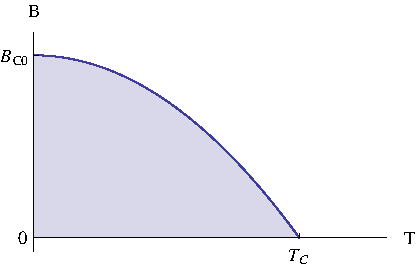
\includegraphics[width=\textwidth]{img/tb0.pdf}
\end{columns}

\end{frame}




\subsection{Two Phases?}
\begin{frame}{Phase Transitions for a Perfect Conductor}

\begin{columns}
\column{.5\textwidth}


\centering \includegraphics<1-2>[height=0.6\textheight]{img/no.pdf}
\includegraphics<3>[height=0.6\textheight]{img/nichdurch.pdf}
\centering \includegraphics<4>[height=0.6\textheight]{img/no.pdf}
\includegraphics<5-6>[height=0.6\textheight]{img/durch.pdf}

 
 
\column{0.5\textwidth}
\includegraphics<1>[width=0.8\textwidth]{img/tb1.pdf}
\includegraphics<2>[width=0.8\textwidth]{img/tb4.pdf}
\includegraphics<3>[width=0.8\textwidth]{img/tb5.pdf}
\includegraphics<4>[width=0.8\textwidth]{img/tb1.pdf}
\includegraphics<5>[width=0.8\textwidth]{img/tb2.pdf}                    
\includegraphics<6>[width=0.8\textwidth]{img/tb3.pdf}

\end{columns}
\end{frame}


\subsection{Meißner-Ochsenfeld Effect}
\begin{frame}{Phase Transitions for a Perfect Conductor}

\begin{columns}
\column{.5\textwidth}
\includegraphics<1>[width=0.25\textheight]{img/durch.pdf}
\includegraphics<1>[width=0.25\textheight]{img/nichdurch.pdf}
 
 
\column{0.5\textwidth}

\includegraphics<1>[width=0.8\textwidth]{img/tb6.pdf}

\end{columns}

\begin{alertblock}<1>{ Are there two different Superconductor-States?}
 
\end{alertblock}

\end{frame}
% Meißner Ochsenfeld -> picture of balls
%		chi diagram
% -> london eqs?




\subsection{Meißner-Ochsenfeld} %2-3 %c

\begin{frame}{Meißner-Ochsenfeld Effect}
\begin{columns}
\column{.5\textwidth}
\includegraphics<1>[width=0.25\textheight]{img/nichdurch.pdf}
\includegraphics<1>[width=0.25\textheight]{img/nichdurch.pdf}
 
 
\column{0.5\textwidth}

\includegraphics<1>[width=0.8\textwidth]{img/tb6.pdf}

\end{columns}

\begin{alertblock}{ Are there two different Superconductor-States?}
 No, because a superconductor is much more then a perfect conductor. It's a new state of matter.
\end{alertblock}
\end{frame}

\begin{frame}{Meißner-Ochsenfeld Effect}
\begin{columns}
\column{.5\textwidth}
\begin{itemize}[<+->]
\item Meißner-Ochsenfeld Effect (1933)
\item Magnetic Field Expulsion $B=\mu H=0$
\item Magnetic Permeability $\mu = \mu_0 ( 1+ \chi) =0$
\item Magnetic Susceptibility $\chi=-1$
\end{itemize}
 
\column{0.5\textwidth}

\includegraphics<1->[width=0.5\textwidth]{img/nichdurch.pdf}

\end{columns}


\end{frame}










\section{BCS Theory} %3-4 %b
\subsection{BCS}
\begin{frame} \frametitle{Slow Electrons}
\begin{columns}
\column{0.55\textwidth}
	\begin{itemize}
		\item<1-> very low temperature $\Rightarrow$ movement of electrons and nucleons on same timescale
		\item<2-> Coulomb interaction causes nucleons to move in direction of the electron
		\item<3-> retarded nucleons create a virtual positive charge "behind" the electron
		\item<4-> electron-electron interactions now include an attractive term!
	\end{itemize} 
\column{0.45\textwidth}
	\includegraphics<1|trans:0>[width=\textwidth]{img/e0.pdf}
	\includegraphics<2|trans:0>[width=\textwidth]{img/e1.pdf}
	\includegraphics<3|trans:0>[width=\textwidth]{img/e2.pdf}
	\includegraphics<4->[width=\textwidth]{img/e3.pdf}
\end{columns}
\end{frame}
%-------------------------------------------------------------------------------
\begin{frame} \frametitle{Cooper Pairs}
\begin{columns}
\column{0.45\textwidth}
	\includegraphics<1->[width=\textwidth]{img/cooper.pdf}
%	\includegraphics<2->[width=\textwidth]{img/deformation.png}
\column{0.55\textwidth}
	\begin{itemize}
		\item<1-> electrons now form "dipoles" that may attract or repel other similar electrons 
		\item<2-> forming pseudo-bound states (with finite lifetime), interacting via phonons
		\item<3-> such a pair is called cooper pair, a new pseudoparticle with
		\begin{itemize}
			\item<4-> a single wavefunction for whole cooper pair
			\item<5-> total spin 0 $\Rightarrow$ bosons!
		\end{itemize}
	\end{itemize} 
\end{columns}
\end{frame}
%-------------------------------------------------------------------------------
\begin{frame} \frametitle{Consequences}
\begin{columns}
\column{1.00\textwidth}
	\begin{itemize}[<+->]
		\item conducting particles - bosons - may all be in the same conducting state without causing further scattering
		\item energies $>$ "binding energy" of cooper pairs will destroy them
		\begin{itemize}
			\item high currents
			\item high magnetic fields
			\item "high" temperatures %TODO picture?
		\end{itemize}
		\item different isotopes of the same element require different temperatures for superconductance
	\end{itemize} 
\begin{block}{ }<7->
	All these effects agree with the experiments!
\end{block}
\end{columns}
\end{frame}
% classical explanation -> pictures, yay!
% isotop effects
% bosonen! -> leitende objekte bla
% Tc, Bc erkl�ren durch ben�tigte energie zum l�sen der paare

\section{Statistics} % 3 %b
\subsection{stats}
\begin{frame} \frametitle{Fermi and Bose Statistics}
\begin{columns}
\column{0.55\textwidth}
	\begin{itemize}
		\item<1-> a (regular) conductor can be approximated using a model of a \emph{free electron gas}
		\item<2-> due to the pauli exclusion principle any two states differ by at least one quantum number $\Rightarrow$ Fermi statistic
		\item<3-> as some electrons become bosonic cooper pairs, they can occupy the same state several times $\Rightarrow$ Bose statistic?
	\end{itemize} 
\column{0.45\textwidth}
	\includegraphics<1-2|trans:0>[width=\textwidth]{img/stat02.pdf}
	\includegraphics<3->[width=\textwidth]{img/stat12.pdf}
\end{columns}
\end{frame}
%-------------------------------------------------------------------------------
\begin{frame} \frametitle{Energy Gap}
\begin{columns}
\column{0.55\textwidth}
	\begin{itemize}
		\item<1-> only about 10\% of all electrons are bound in cooper pairs
		\item<2-> pairs can only be created near the Fermi energy and have a finite lifetime
		\item<3-> thus the density of states increases mainly near the Fermi energy
		\item<4-> an energy gap is created corresponding to the energy required  to create a cooper pair ($=2\Delta$)
	\end{itemize} 
\column{0.45\textwidth}
	\includegraphics<1-2|trans:0>[width=\textwidth]{img/f0.pdf}
	\includegraphics<3->[width=\textwidth]{img/f1.pdf}
\end{columns}
\end{frame}
%-------------------------------------------------------------------------------

% fermi, boson, statistics
% free electron gas?
% energy gap






\section{Experiment}
\subsection{Overview} %2 %c
% what we want to measure -> Tc, Bc ~ Tc^2
\begin{frame}{Measurements}
\begin{columns}
\column{.5\textwidth}
\begin{itemize}[<+->]
\item Indium and Tin
\item $T_C$, $B_C(T)$, $B_{C0}$
\item via magnetic property $\chi_c=-1$
\end{itemize}
\column{.5\textwidth}
\includegraphics<1>[width=0.4\textwidth]{img/indium.JPG}
\hfill
\includegraphics<1>[width=0.4\textwidth]{img/tin.JPG}
\vfill
\includegraphics<2>[width=\textwidth]{img/tb0.pdf}
\includegraphics<3>[width=0.7\textwidth]{img/nichdurch.pdf}
\end{columns}
\footnotetext[1]{\tiny \url{http://periodictable.com}}
\end{frame}


\subsection{Setup} %2 %c
\begin{frame}{Experimental Set-Up}
\begin{columns}
\column{.5\textwidth}
\begin{figure}
\centering
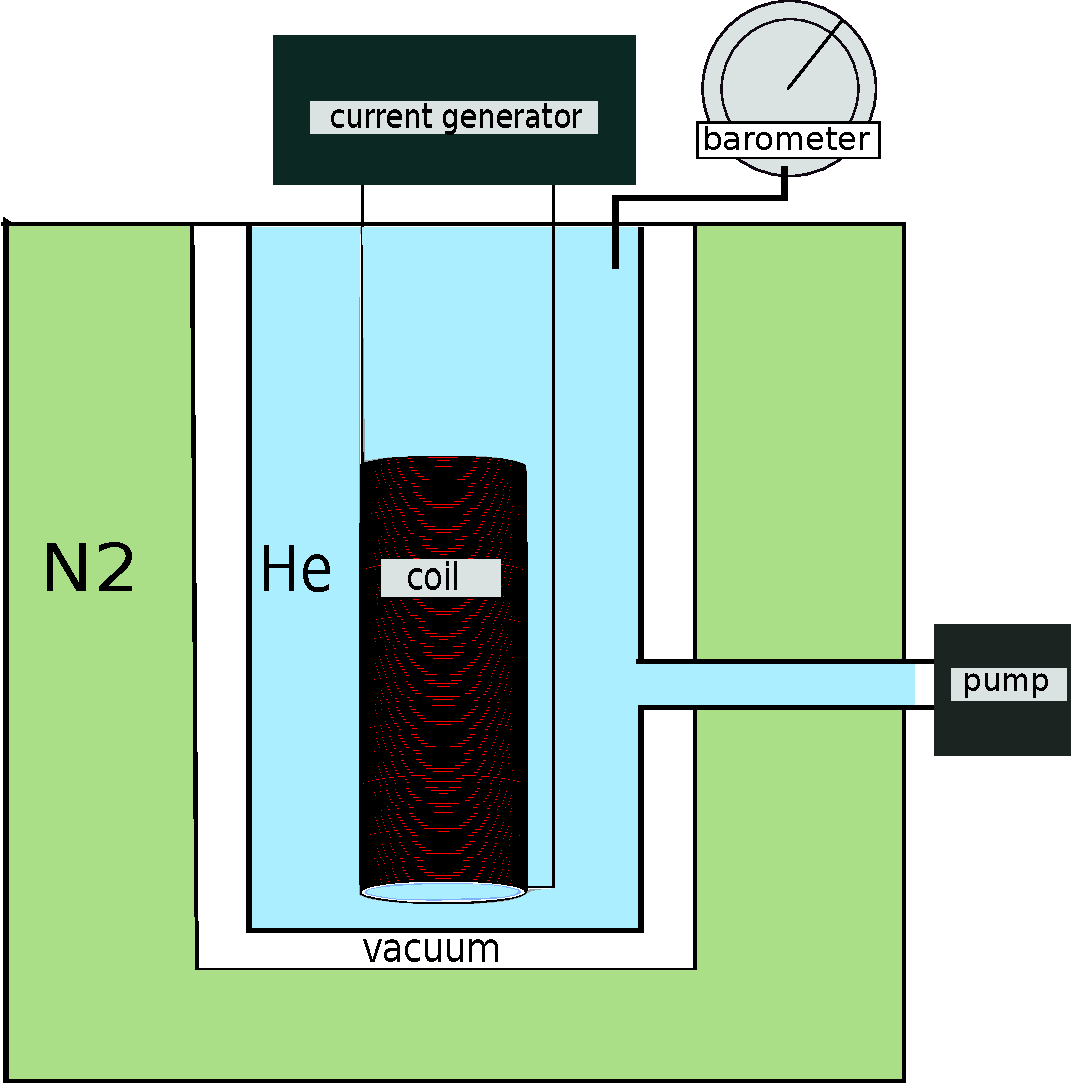
\includegraphics[height=0.6\textheight]{img/Zeichnung.pdf}
\end{figure}
\column{.5\textwidth}
\begin{itemize}[<+->]
\item two level cooling chamber
\item tune temperature via He pressure
\item tune magnetic field via current
\item inside coil -- induction system
\end{itemize}
\end{columns}

\end{frame}


\subsection{Setup} %2 %c
\begin{frame}{Experimental Set-Up}
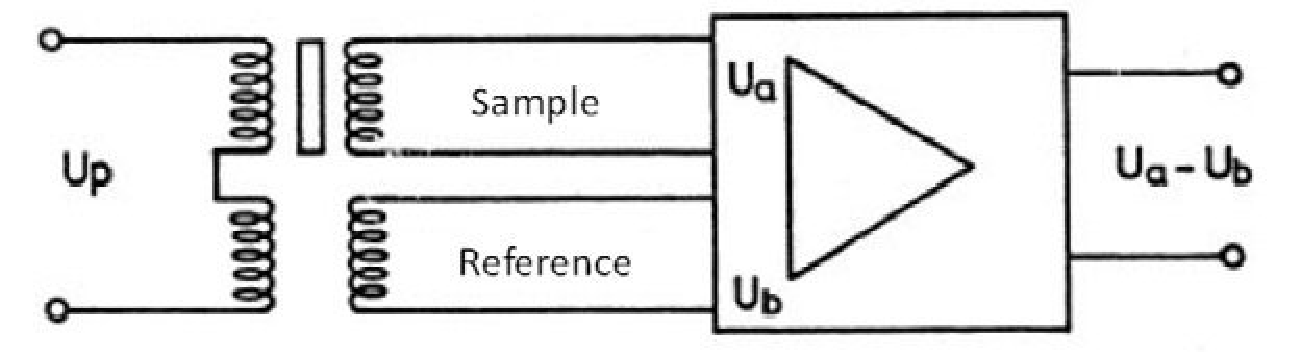
\includegraphics[height=0.2\textheight]{img/detail.pdf}
\begin{itemize}[<+->]
\item working principle of a transformer
\item induction voltage $U = \frac{\mathrm{d}\Phi}{\mathrm d t} $
\item magnetic flux $\Phi \sim \mu H$
\item $\mu=0$ or $\chi=-1$ for superconducting phase
\item $U_a \ll U_b$ for $T<T_c$ and $B<B_c$
\end{itemize}



\end{frame}

% kammern, khlung
% messgleichung?
% druck -> T








\subsection{Result} %3 %b
% expected T-Chi-curve
% Bc-T-Diagram -> bc0
% Values for Sn, T

\section{Outlook} %1
% hochtemp. supraleiter
% organische supraleiter??
% FB

% aufgabe c,d wissen. formeln?

\section[Sources]{References}
\begin{frame} \frametitle{Sources \& Literature}
\nocite{buckel}
\nocite{tinkham}
\nocite{BCS}
\nocite{GL}
\nocite{hofmann}
\bibliographystyle{unsrt}
\bibliography{bib}
\end{frame}





\end{document}

%------------------------------------------------
% usage:
%------------------------------------------------
%\subsection{Knstliches Leben}\textbf{•}
%\begin{frame}\frametitle{Knstliches Leben}
%\begin{itemize}
%	\item<2-> Erste Anwendungen simulierten Knstliches Leben um das echte Leben 
%			zu erforschen
%	\item<3-> Fragestellungen vorgegeben durch Evolutionstheorie der vergangenen %Jahre: 
%\begin{itemize}
%		\item<4-> Balz 
%		\item<5-> Geschlechter
%		\item<6-> haploid vs. diploid
%		\item<7-> Introns
%	\end{itemize}
%\end{itemize}
%\end{frame}

%------------------------------------------------
% useful blocks
%------------------------------------------------
%\begin{block}{Blocktitel}
% Blocktext 
%\end{block}
%
%\begin{exampleblock}{Blocktitel}
% Blocktext 
%\end{exampleblock}
%
%
%\begin{alertblock}{Blocktitel}
% Blocktext 
%\end{alertblock}
